\begin{frame}[c]{Where are we? The big picture}

\begin{itemize}
\item Algorithm Selection
  \begin{itemize}
    \item Portfolios
    \item Algorithm selection (for runtime)
  \end{itemize}
  \item Design decisions:\\ Local Search + Evo. Algorithms + Machine Learning 
  \item Empirical evaluation
  \item[$\to$] AAD for ML
  \begin{itemize}
    \item Hyperparameter optimization and Bayesian optimization 
    \item[$\to$] AutoML \& Neural architecture search (lecture given by Prof. Hutter)
  \end{itemize}
  \item Algorithm configuration 
  \begin{itemize}
    \item Basics 
    \item State of the art 
    \item Best practices 
  \end{itemize}
  \item Combinations of algorithm selection and configurations
  \item Algorithm control 
  \item Algorithm analysis 
  \item Project announcement and questions for exam 
\end{itemize}

\end{frame}
%----------------------------------------------------------------------
%----------------------------------------------------------------------
\begin{frame}[c]{}

\huge
\centering
AutoML \& Neural Architecture Search

\end{frame}
%----------------------------------------------------------------------
\begin{frame}[c]{Learning Goals}

\begin{itemize}
	\item After this lecture, you can ...
	\begin{itemize}
		\item explain how AutoML can be formulated as a hyperparameter
		optimization problem
		\item list various contemporary HPO methods, along with advantages
		and disadvantages
		\item describe how to use multi-fidelity methods to speed up HPO
		\item describe different search spaces for neural architecture search
		\item describe various blackbox optimization methods for NAS
		\item explain various speedup techniques for NAS
	\end{itemize}
\end{itemize}
\end{frame}
%----------------------------------------------------------------------
{\setbeamertemplate{logo}{}
\begin{frame}[c]{Motivation: Success of Deep Learning}
\centering
\includegraphics[width=\textwidth]{images/lecture_frank/s1}
\end{frame}
}
%----------------------------------------------------------------------
%----------------------------------------------------------------------
%{\setbeamertemplate{logo}{}
\begin{frame}[c]{One Problem of Deep Learning}
\centering
\includegraphics[width=\textwidth]{images/lecture_frank/s2}
\end{frame}
%}
%----------------------------------------------------------------------
{\setbeamertemplate{logo}{}
	\begin{frame}[c]{Deep learning and AutoML}
	\centering
	\includegraphics[width=.9\textwidth]{images/lecture_frank/s3}
\end{frame}
}
%----------------------------------------------------------------------
{\setbeamertemplate{logo}{}
\begin{frame}[c]{Deep Reinforcement Learning and AutoML}
\centering
\includegraphics[width=.9\textwidth]{images/lecture_frank/s4}
\end{frame}
}
%----------------------------------------------------------------------
\begin{frame}[c]{Benchmark for Progress: AutoML Challenge}
\begin{itemize}
	\item \alert{Large-scale challenge run by ChaLearn \& CodaLab}
	\begin{itemize}
		\item 17 months, 5 phases with 5 new datasets each (2015-2016)
		\item 2 tracks: code submissions / Kaggle-like human track
	\end{itemize}
	\item \alert{Code submissions: true end-to-end learning necessary}
	\begin{itemize}
		\item Get training data, learn model, make predictions for test data
		\item 1 hour end-to-end
	\end{itemize}
	\item \alert{25 datasets from wide range of application areas}
		\begin{itemize}
			\item Already featurized
			\item Inputs: features $X$, targets $y$
		\end{itemize}
\end{itemize}
\end{frame}
%----------------------------------------------------------------------
%----------------------------------------------------------------------
\begin{frame}[c]{Outline}
\begin{itemize}
	\item Modern Hyperparameter Optimization
	\begin{itemize}
		\item[$\to$] AutoML as Hyperparameter Optimization
		\item Blackbox optimization
		\item AutoML Systems based on BlackBox Optimization
		\item Beyond Blackbox Optimization 
	\end{itemize}
	\item Neural Architecture Search
	\begin{itemize}
		\item Brief History
		\item Search Space Design
		\item Blackbox Optimization
		\item Beyond Blackbox Optimization
	\end{itemize}
\end{itemize}
\end{frame}
%----------------------------------------------------------------------
%----------------------------------------------------------------------
{\setbeamertemplate{logo}{}
\begin{frame}[c]{Hyperparameter Optimization}
Let's recap the definition
\begin{block}{Definition: Hyperparameter Optimization (HPO)}
	Let
	\begin{itemize}
		\item $\vlambda$ be the hyperparameters of a ML algorithm $A$ with domain $\vLambda$,
		\item $D_{opt}$ be a training set which is split into $D_{train}$ and $D_{valid}$
		\item \alert{$\mathcal{L}(A_{\vlambda}, D_{train}, D_{valid})$} denote the loss of $A$, using hyperparameters $\vlambda$ trained on $D_{train}$ and evaluated on $D_{valid}$.
	\end{itemize}
	The \alert{hyperparameter optimization (HPO)} problem is to find a hyperparameter configuration $\vlambda^*$ that minimizes this loss:
	
	\begin{equation}
	\alert{\vlambda^* \in \argmin_{\vlambda \in \vLambda} \mathcal{L}(A_{\vlambda}, D_{train}, D_{valid})} \nonumber 
	\end{equation}
	
\end{block}

\end{frame}
}
%----------------------------------------------------------------------
%----------------------------------------------------------------------
{\setbeamertemplate{logo}{}
\begin{frame}[c]{The CASH Formulation of AutoML}

\begin{block}{Definition: Combined Algorithm Selection and Hyperparameter Optimization (CASH)}
Let
\begin{itemize}
	\item $\mathcal{A} = \{ A^{(1)}, \dots, A^{(n)} \}$ be a set of algorithms with
	\item $\vLambda^{(i)}$ be the hyperparameter space of $A^{(i)}$, for $i=1, \dots, n$
	\item \alert{$\mathcal{L}(A^{(i)}_{\vlambda}, D_{train}, D_{valid})$} denote the loss of $A^{(i)}$, using $\lambda \in \vLambda^{(i)}$ trained on $D_{train}$ and evaluated on $D_{valid}$.
\end{itemize}
The \alert{Combined Algorithm Selection and Hyperparameter Optimization (CASH)} problem is to find a combination of algorithm $A^*=A^{(i)}$ and hyperparameter configuration $\vlambda^* \in \vLambda^{(i)}$ that minimizes this loss:

\begin{equation}
\alert{A^*_{\vlambda^*} \in \argmin_{A^{(i)} \in \mathcal{A}, \vlambda \in \vLambda^{(i)}} \mathcal{L}(A^{(i)}_{\vlambda}, D_{train}, D_{valid})} \nonumber 
\end{equation}

\end{block}
\end{frame}
}
%----------------------------------------------------------------------
%----------------------------------------------------------------------

\begin{frame}[c]{Types of Hyperparameters}
\begin{itemize}
	\item Continuous
	\begin{itemize}
		\item E.g., learning rate
	\end{itemize}
	\item Integer
	\begin{itemize}
		\item E.g, \#units
	\end{itemize}
	\item Ordinal
	\begin{itemize}
		\item E.g, L0, L1, L2 regularization
	\end{itemize}
	\item \alert{Categorical}
	\begin{itemize}
		\item Finite domain, unordered
		\item E.g., choice between \{SVM, RF, NN\}
		\item E.g., choice between \{ReLU, ELU, tanh\}
		\item E.g., choice between \{conv3x3, conv5x5, max pool, separable conv3x3, $\ldots$\}
		\item Special case: binary
	\end{itemize}
\end{itemize}
\end{frame}
%----------------------------------------------------------------------
%----------------------------------------------------------------------

\begin{frame}[c]{Conditional Hyperparameters}
\begin{itemize}
	\item Some hyperparameters B are only active if another
	hyperparameter A is set a certain way
	\begin{itemize}
		\item Example 1:
		\begin{itemize}
			\item A = choice of optimizer (Adam or SGD)
			\item B = Adam‘s second momentum hyperparameter\\
			This is provably unimportant (not inspected) unless Adam is selected
		\end{itemize}
		\item Example 2:
		\begin{itemize}
			\item A = number of layers
			\item B = weight decay for layer 10\\
			This is only active if A >= 10
		\end{itemize}
	\end{itemize}
	\item Hyperparameters give rise to a \alert{structured space of algorithms}
	\begin{itemize}
		\item Many \alert{configurations} (e.g. $10^{47}$)
		\item Configurations often yield qualitatively different behaviour
	\end{itemize}
\end{itemize}
\end{frame}
%----------------------------------------------------------------------
%----------------------------------------------------------------------
{\setbeamertemplate{logo}{}
	\begin{frame}[c]{AutoML as Hyperparameter Optimization}
	
	\begin{block}{Definition: Combined Algorithm Selection and Hyperparameter Optimization (CASH)}
		Let
		\begin{itemize}
			\item $\mathcal{A} = \{ A^{(1)}, \dots, A^{(n)} \}$ be a set of algorithms with
			\item $\vLambda^{(i)}$ be the hyperparameter space of $A^{(i)}$, for $i=1, \dots, n$
			\item \alert{$\mathcal{L}(A^{(i)}_{\vlambda}, D_{train}, D_{valid})$} denote the loss of $A^{(i)}$, using $\lambda \in \vLambda^{(i)}$ trained on $D_{train}$ and evaluated on $D_{valid}$.
		\end{itemize}
		The \alert{Combined Algorithm Selection and Hyperparameter Optimization (CASH)} problem is to find a combination of algorithm $A^*=A^{(i)}$ and hyperparameter configuration $\vlambda^* \in \vLambda^{(i)}$ that minimizes this loss:
		
		\begin{equation}
		\alert{A^*_{\vlambda^*} \in \argmin_{A^{(i)} \in \mathcal{A}, \vlambda \in \vLambda^{(i)}} \mathcal{L}(A^{(i)}_{\vlambda}, D_{train}, D_{valid})} \nonumber 
		\end{equation}
		
	\end{block}
$\Rightarrow$ Simply a HPO problem with a top-level hyperparameter\\
(choice of algorithm) that all other hyperparameters are conditional on
\end{frame}
}
%----------------------------------------------------------------------
%----------------------------------------------------------------------
\begin{frame}[c]{AutoML as Hyperparameter Optimization}
\begin{itemize}
	\item Pipeline Optimization as Hyperparameter Optimization:
	\begin{itemize}
		\item Clean \& preprocess the data
		\item Select / engineer better features
		\item Select a model family
		\item Set the hyperparameters
		\item Construct ensembles of models
	\end{itemize}
	\item Joint Neural Architecture and Hyperparameter Search
	\begin{itemize}
		\item Architectural Hyperparameters
		\item “Standard” Hyperparameters
	\end{itemize}
\end{itemize}
\end{frame}
%----------------------------------------------------------------------
%----------------------------------------------------------------------
\begin{frame}[c]{Manual step left: setting the ranges}
\begin{itemize}
	\item What domain should we search in?
	\begin{itemize}
		\item Too broad: most hyperparameter configurations are very poor
		\item Too narrow: may not include optimal configuration
	\end{itemize}
	\item One may want to set hyperparameters as a function of
	\begin{itemize}
		\item The layer (e.g., learning rates, regularization)
		\item The training epoch\\
		(e.g., learning rate schedule, increasing regularization)
	\end{itemize}
\end{itemize}
\end{frame}
%----------------------------------------------------------------------
%----------------------------------------------------------------------
\begin{frame}[c]{Outline}
\begin{itemize}
	\item Modern Hyperparameter Optimization
	\begin{itemize}
		\item AutoML as Hyperparameter Optimization
		\item[$\to$] Blackbox optimization
		\item AutoML Systems based on BlackBox Optimization
		\item Beyond Blackbox Optimization 
	\end{itemize}
	\item Neural Architecture Search
	\begin{itemize}
		\item Brief History
		\item Search Space Design
		\item Blackbox Optimization
		\item Beyond Blackbox Optimization
	\end{itemize}
\end{itemize}
\end{frame}
%----------------------------------------------------------------------
%----------------------------------------------------------------------
\begin{frame}[c]{Blackbox Hyperparameter Optimization}
	\centering
	\includegraphics[width=.9\textwidth]{images/lecture_frank/s5}
\end{frame}
%----------------------------------------------------------------------
%----------------------------------------------------------------------
\begin{frame}[c]{AutoML Challenges for Bayesian Optimization}
\begin{itemize}
	\item Problems for standard Gaussian Process (GP) approach:
	\begin{itemize}
		\item \alert{Complex hyperparameter space}
		\begin{itemize}
			\item High-dimensional (low effective dimensionality)
			\item Mixed continuous/discrete hyperparameters
			\item Conditional hyperparameters
			\item Discrete change points
		\end{itemize}
		\item \alert{Noise}: sometimes heteroscedastic, large, non-Gaussian
		\item \alert{Robustness} (usability out of the box)
		\item Model \alert{overhead} (budget is runtime, not \#function evaluations)
	\end{itemize}
	\item You saw one simple solution: \alert{random forests} \lit{Breiman, '01}
	\begin{itemize}
		\item Adapted to yield uncertainty estimates
		as a mixture model over trees
	\end{itemize}
\end{itemize}
\end{frame}
%----------------------------------------------------------------------
%----------------------------------------------------------------------
\begin{frame}[c]{Comparing Bayesian Hyperparameter Optimizers}
\vspace*{-2cm}
{\centering\lit{Eggensperger, Feurer, Hutter, Bergstra, Snoek, Hoos \& Leyton-Brown, BayesOpt 2013}}
%\vspace*{2cm}
\begin{itemize}
	\item Hyperparameter optimization library: \url{automl.org/hpolib}
	\begin{itemize}
		\item \alert{Benchmarks}
		\begin{itemize}
			\item From 2-dimensional continuous hyperparameter spaces
			\item To structured ones with 768 hyperparameters
		\end{itemize}
		\item \alert{Optimizers}
		\begin{itemize}
			\item SMAC \lit{Hutter et al, '11} , based on random forests
			\item Spearmint \lit{Snoek et al, '12} , based on Gaussian processes
			\item TPE \lit{Bergstra et al, '11} , based on 1-d distributions of good values
		\end{itemize}
	\end{itemize}
	\item Results
	\begin{itemize}
		\item GP-based Spearmint is best for \alert{low-dimensional \& continuous}
		\item RF-based SMAC is best for high-dim, \alert{categorical \& conditional}
	\end{itemize}
\end{itemize}
\end{frame}
%----------------------------------------------------------------------
%----------------------------------------------------------------------
{\setbeamertemplate{logo}{}
\begin{frame}[c]{Neural networks to the rescue?}
\begin{itemize}
	\item Two recent promising models for Bayesian optimization
	\begin{itemize}
		\item Neural networks with Bayesian linear regression
		using the features in the output layer \lit{Snoek et al, ICML 2015}
		\item Fully Bayesian neural networks, trained with stochastic gradient
		Hamiltonian Monte Carlo \lit{Springenberg et al, NIPS 2016}
	\end{itemize}
\end{itemize}
\begin{minipage}{0.5\textwidth}
	\begin{itemize}
		\item Good performance on low-dimensional HPOlib tasks
		\item So far not studied for:
		\begin{itemize}
			\item High dimensionality
			\item Conditional hyperparameters
		\end{itemize}
	\end{itemize}
\end{minipage}
\begin{minipage}{0.49\textwidth}
	\centering
	\includegraphics[width=\textwidth]{images/lecture_frank/s6}
\end{minipage}
\end{frame}
}
%----------------------------------------------------------------------
%----------------------------------------------------------------------
\begin{frame}[c]{Estimation of Distribution (EDA) Algorithms}
\begin{itemize}
	\item Categorize performance into good and bad, and fit a
	model (density estimator) of the good points in the
	space: \alert{P(x is “good”)}
	\begin{itemize}
		\item Often: independent Gaussians for each dimension
	\end{itemize}
	\item Sample next point to evaluate from the model
\end{itemize}
{\centering
	\includegraphics[width=\textwidth]{images/lecture_frank/s7}
	Image source: Wikipedia
}
\end{frame}
%----------------------------------------------------------------------
%----------------------------------------------------------------------
\begin{frame}[c]{Population-based Methods}
\begin{itemize}
	\item Population of configurations
	\begin{itemize}
		\item Global + local search via population
		\item Maintain population \alert{fitness \& diversity}
	\end{itemize}
	\item Examples
	\begin{itemize}
		\item Genetic algorithms \lit{e.g., Barricelli, ’57, Goldberg, ’89}
		\item Evolutionary strategies \lit{e.g., Beyer \& Schwefel, ’02}
	\end{itemize}
	\item Covariance matrix adaptation evolutionary strategy (CMA-ES)
	\begin{itemize}
		\item Highly competitive for optimizing continuous hyperparameters of
		deep neural networks \lit{Loshchilov \& Hutter, ‘16}
		\item Especially when we can optimize on many machines in parallel
	\end{itemize}
\end{itemize}
\end{frame}
%----------------------------------------------------------------------
%----------------------------------------------------------------------
\begin{frame}[c]{Outline}
\begin{itemize}
	\item Modern Hyperparameter Optimization
	\begin{itemize}
		\item AutoML as Hyperparameter Optimization
		\item Blackbox optimization
		\item[$\to$] AutoML Systems based on BlackBox Optimization
		\item Beyond Blackbox Optimization 
	\end{itemize}
	\item Neural Architecture Search
	\begin{itemize}
		\item Brief History
		\item Search Space Design
		\item Blackbox Optimization
		\item Beyond Blackbox Optimization
	\end{itemize}
\end{itemize}
\end{frame}
%----------------------------------------------------------------------
%----------------------------------------------------------------------
\begin{frame}[c]{AutoML System 1: Auto-WEKA}

{\centering
	\includegraphics[width=\textwidth]{images/lecture_frank/s8}
}
\begin{itemize}
	\item P\alert{arameterize ML framework: WEKA} \lit{Witten et al, 1999-current}
	\begin{itemize}
		\item 27 base classifiers (with up to 10 hyperparameters each)
		\item 2 ensemble methods; in total: 786 hyperparameters
	\end{itemize}
	\item Optimize \alert{CV performance} by Bayesian optimization (SMAC)
	\begin{minipage}{0.675\textwidth}
		\begin{itemize}
			\item Only evaluate more folds for good configurations
			\begin{itemize}
				\item 5x speedups for 10-fold CV
			\end{itemize}
		\end{itemize}
	\end{minipage}%
	\begin{minipage}{0.26\textwidth}
{\centering
	\includegraphics[width=.9\textwidth]{images/lecture_frank/s9}
}
	\end{minipage}
\end{itemize}
\end{frame}
%----------------------------------------------------------------------
%----------------------------------------------------------------------
\begin{frame}[c]{AutoML System 2: Auto-sklearn}

{\centering
	\includegraphics[width=\textwidth]{images/lecture_frank/s10}
}
\begin{itemize}
	\begin{minipage}{0.55\textwidth}
		\item Optimize CV performance by SMAC
	\end{minipage}
	\begin{minipage}{0.26\textwidth}
		{\centering
			\includegraphics[width=.65\textwidth]{images/lecture_frank/s9}
		}
	\end{minipage}
	\begin{minipage}{0.75\textwidth}
	\item \alert{Meta-learning} to warmstart Bayesian optimization
	\begin{itemize}
		\item Reasoning over different datasets
		\item Dramatically speeds up the search (2 days $\rightarrow$ 1 hour)
	\end{itemize}
	\end{minipage}
	\begin{minipage}{0.15\textwidth}
	{\centering
		\includegraphics[width=.9\textwidth]{images/lecture_frank/s11}
	}
	\end{minipage}
	\item Automated \alert{posthoc ensemble construction}
	to combine the models Bayesian optimization evaluated
		\begin{itemize}
			\item Efficiently re-uses its data; improves robustness
		\end{itemize}
\end{itemize}
\end{frame}
%----------------------------------------------------------------------
%----------------------------------------------------------------------
\begin{frame}[c]{Auto-sklearn: Ready for Prime Time}

{\centering
	\includegraphics[width=\textwidth]{images/lecture_frank/s112}
}
\end{frame}
%----------------------------------------------------------------------
%----------------------------------------------------------------------
\begin{frame}[c]{Auto-sklearn: Ready for Prime Time}

{\centering
	\includegraphics[width=\textwidth]{images/lecture_frank/s112}
}
\end{frame}
%----------------------------------------------------------------------
%----------------------------------------------------------------------
\begin{frame}[c]{Example Application: Robotic Object Handling}
\begin{itemize}
	\begin{minipage}{0.325\textwidth}
		\item Collaboration with Freiburg’s robotics group
		\item Binary classification task for object placement: \alert{will the object fall over?}
	\end{minipage}
	\begin{minipage}{0.575\textwidth}
		{\centering
			\includegraphics[width=.7\textwidth]{images/lecture_frank/s13}
		}
	\end{minipage}
	\item Dataset
	\begin{itemize}
		\item Based on BigBIRD and YCB Object and Model Set
		\item 30000 data points
		\item 50 features -- manually defined \lit{BSc thesis, Hauff 2015}
	\end{itemize}
	\item Performance
	\begin{itemize}
		\item \alert{Caffe deep learning framework: 2\% error rate}
		\item \alert{Auto-sklearn: 0.6\% error rate}(within 30 minutes)
	\end{itemize}
\end{itemize}
\end{frame}
%----------------------------------------------------------------------
%----------------------------------------------------------------------
\begin{frame}[c]{Outline}
\begin{itemize}
	\item Modern Hyperparameter Optimization
	\begin{itemize}
		\item AutoML as Hyperparameter Optimization
		\item Blackbox optimization
		\item AutoML Systems based on BlackBox Optimization
		\item[$\to$] Beyond Blackbox Optimization 
	\end{itemize}
	\item Neural Architecture Search
	\begin{itemize}
		\item Brief History
		\item Search Space Design
		\item Blackbox Optimization
		\item Beyond Blackbox Optimization
	\end{itemize}
\end{itemize}
\end{frame}
%----------------------------------------------------------------------
%----------------------------------------------------------------------
\begin{frame}[c]{Beyond Blackbox Hyperparameter Optimization}

{\centering
	\includegraphics[width=\textwidth]{images/lecture_frank/s14}
}
\end{frame}
%----------------------------------------------------------------------
%----------------------------------------------------------------------
\begin{frame}[c]{Using Cheap Approximations of the Blackbox}
\begin{itemize}
	\item \alert{One possible approximation: use a subset of the data}
	\begin{itemize}
		\item E.g.: SVM on MNIST
		\item Many cheap evaluations on small subsets
		\item Few expensive evaluations on the full data
		\item \alert{Up to 1000x speedups} \lit{Klein et al, AISTATS 2017}
	\end{itemize}
\end{itemize}
{\centering
	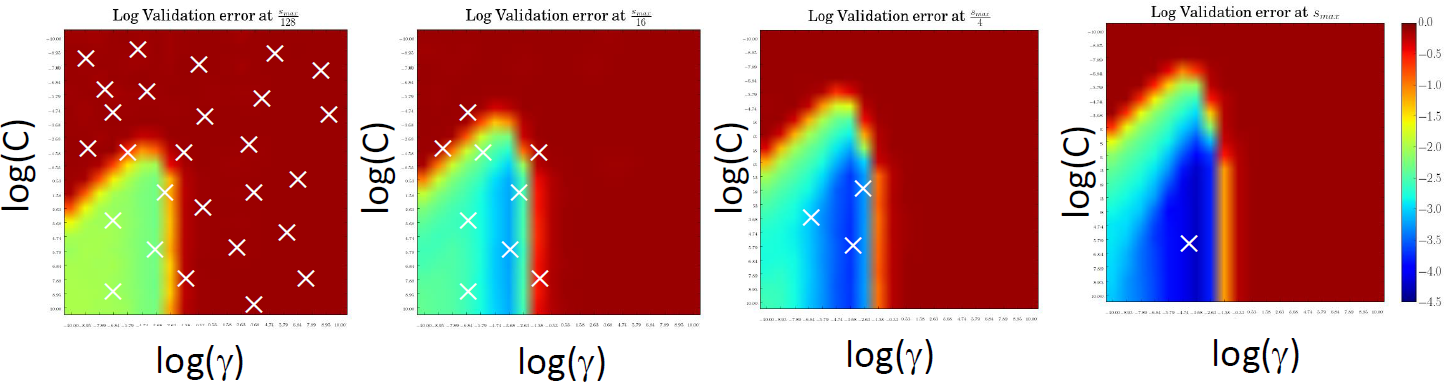
\includegraphics[width=\textwidth]{images/lecture_frank/MNIST}
}
\end{frame}
%----------------------------------------------------------------------
%----------------------------------------------------------------------
\begin{frame}[c]{Using Cheap Approximations of the Blackbox}
\begin{itemize}
	\item \alert{One possible approximation: use less epochs of SGD}
	\begin{itemize}
		\item \lit{Swersky et al, arXiv 2014; Domhan et al, IJCAI 2015}
	\end{itemize}
\end{itemize}
{\centering
	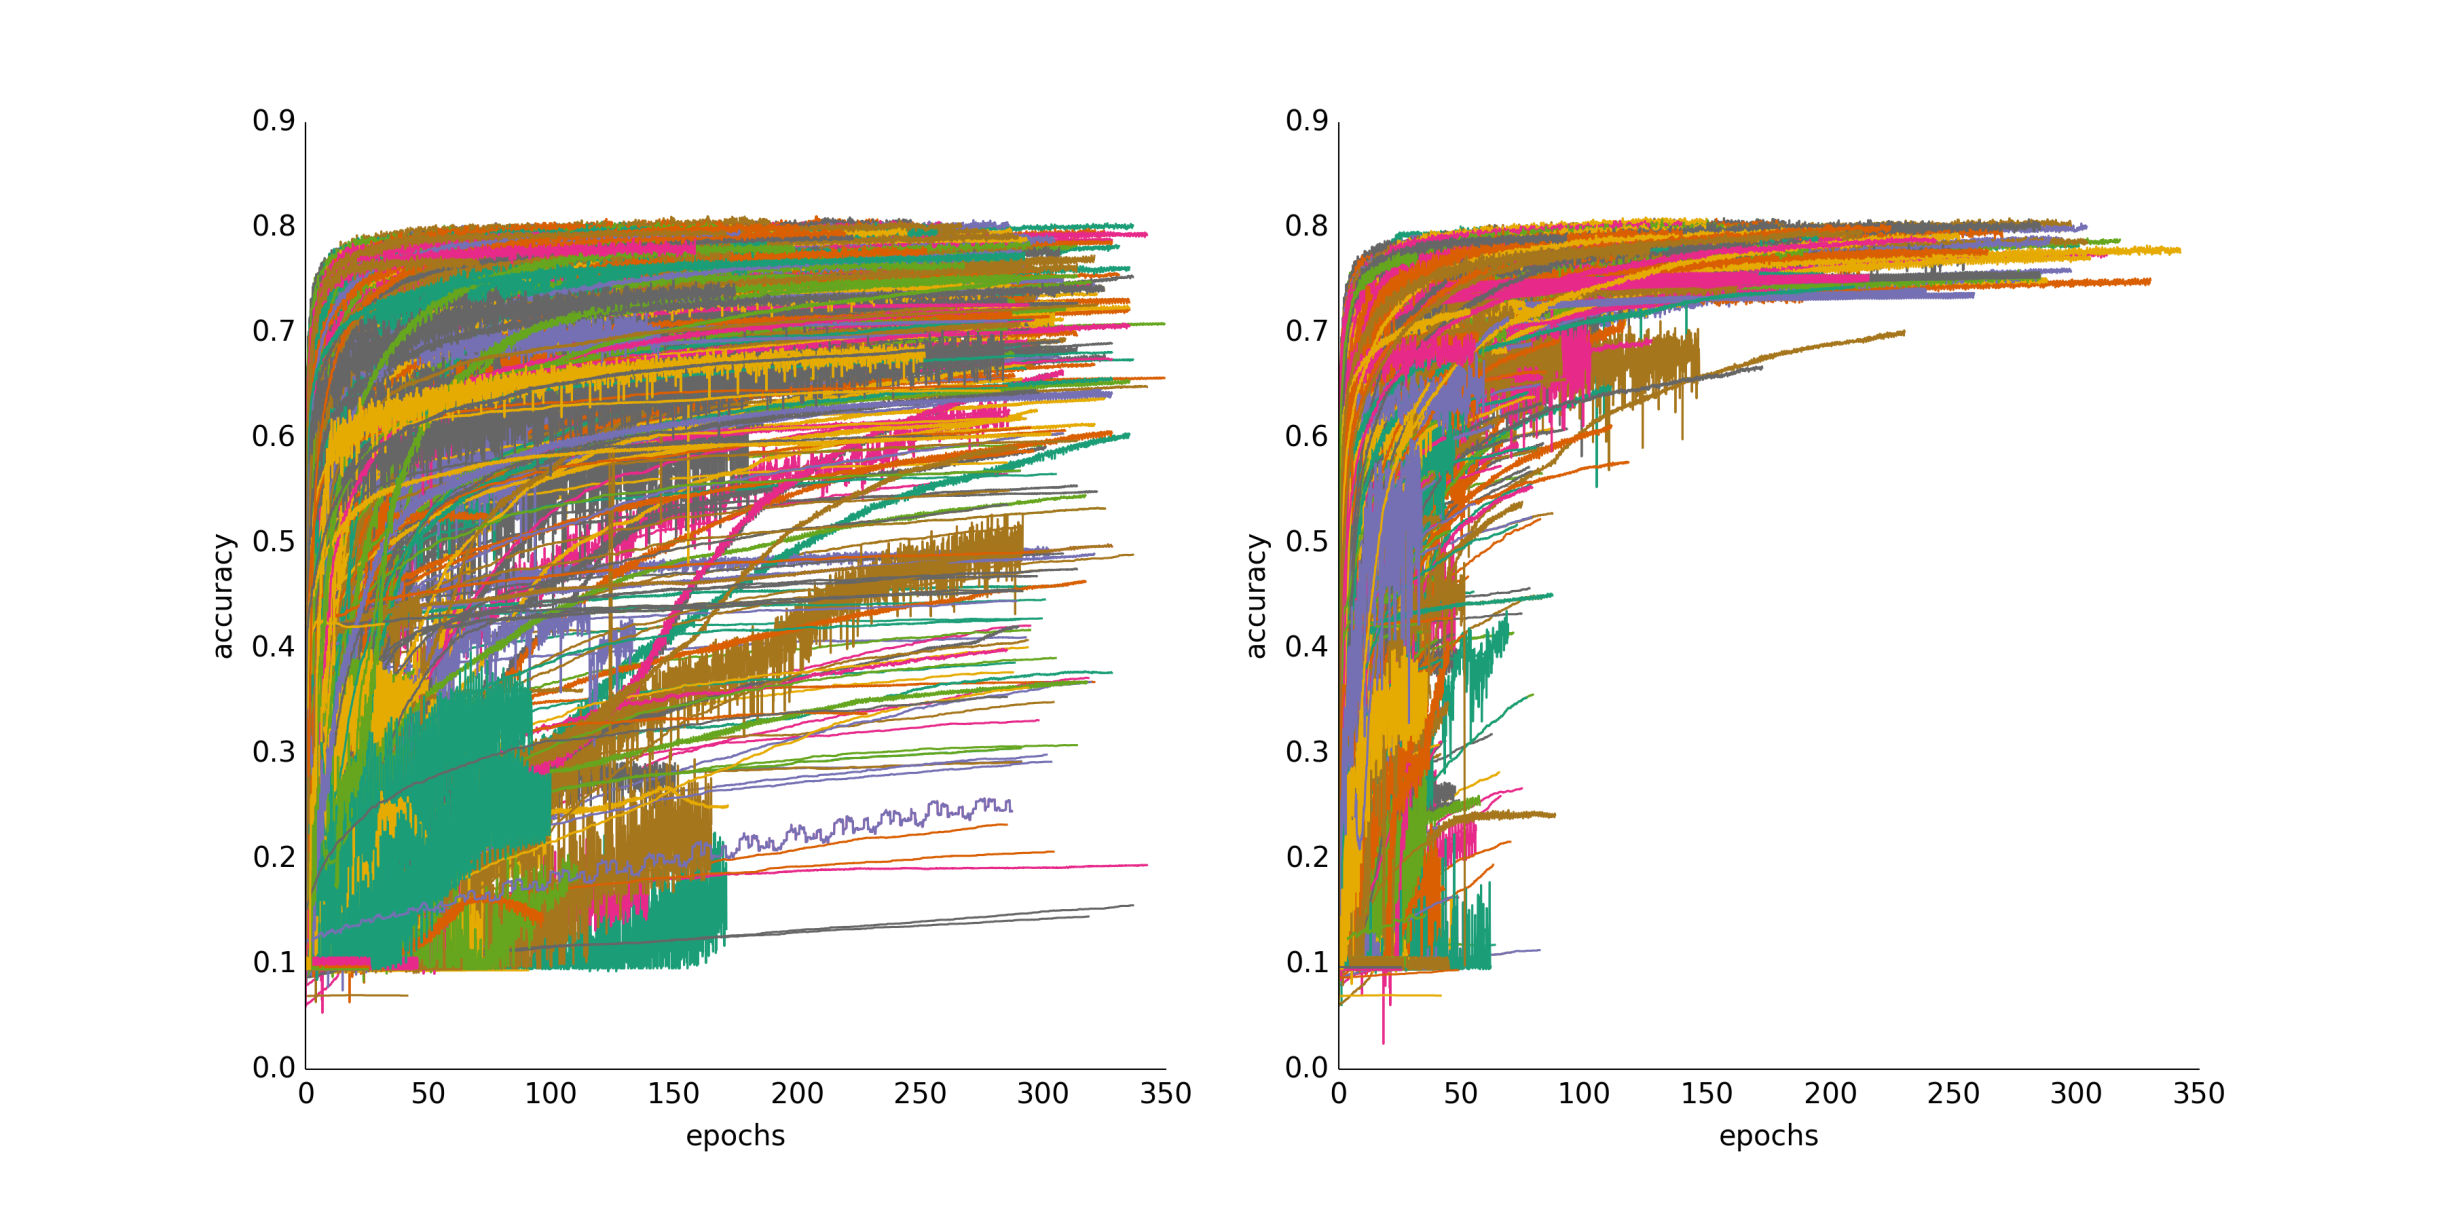
\includegraphics[width=\textwidth]{images/learning_curve_tuning}
	All learning curves vs. Learning curves with early termination
}
\end{frame}
%----------------------------------------------------------------------
%----------------------------------------------------------------------
\begin{frame}[c]{Using Cheap Approximations of the Blackbox}
\begin{itemize}
	\item \alert{Cheap approximations exist in many applications}
	\begin{itemize}
		\item Subset of data
		\item Fewer epochs of iterative training algorithms (e.g., SGD)
		\item Downsampled images in object recognition
		\item Shorter MCMC chains in Bayesian deep learning
		\item Fewer trials in deep reinforcement learning
	\end{itemize}
	\item Also applicable in different domains, e.g., fluid simulations:
	\begin{itemize}
		\item Less particles
		\item Shorter simulations
	\end{itemize}
\end{itemize}
\end{frame}
%----------------------------------------------------------------------
%----------------------------------------------------------------------
\begin{frame}[c]{How to Exploit Cheap Approximations}
\begin{itemize}
	\item \alert{Bayesian optimization} \lit{Klein et al, 2017; Kandasamy et al, 2017}
	\begin{itemize}
		\item Fit a predictive model $f(\lambda,b)$ to predict performance as a
		function of hyperparameters $\lambda$ and budget b
		\item Extrapolate performance from small to large budgets
	\end{itemize}
	\item \alert{Simpler approach}:
	\begin{itemize}
		\item Successive Halving \lit{Jamieson \& Talwalkar, AISTATS 2015}
		\item Hyperband \lit{Li et al, ICLR 2017}
	\end{itemize}
\end{itemize}
{\centering
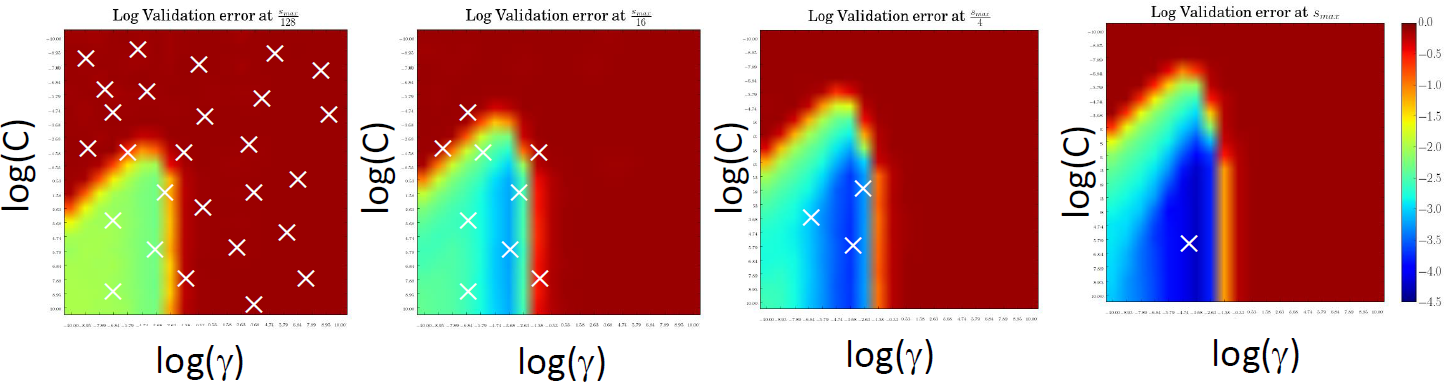
\includegraphics[width=\textwidth]{images/lecture_frank/MNIST}
}
\end{frame}
%----------------------------------------------------------------------
%----------------------------------------------------------------------
\begin{frame}[c]{BOHB: Bayesian Optimization \& Hyperband}
\vspace*{-1.65cm}
\lit{Falkner, Klein \& Hutter, ICML 2018}
\begin{itemize}
	\item \alert{Bayesian optimization}
	\begin{itemize}
		\item for choosing the configuration to evaluate
	\end{itemize}
	\item \alert{Hyperband}:
	\begin{itemize}
		\item for deciding how to allocate budgets
	\end{itemize}
	\item \alert{Advantages}
	\begin{itemize}
		\item Strong performance
		\item General-purpose
		\begin{itemize}
			\item Low-dimensional continuous spaces
			\item High-dimensional spaces with conditionality, categorical dimensions, etc
		\end{itemize}
		\item Easy to implement
		\item Scalable
		\item Easily parallelizable
	\end{itemize}
\end{itemize}
\end{frame}
%----------------------------------------------------------------------
%----------------------------------------------------------------------
{\setbeamertemplate{logo}{}
\begin{frame}[c]{Hyperband vs. Random Search}

{\centering
	\includegraphics[width=\textwidth]{images/lecture_frank/s15}
}
\end{frame}
}
%----------------------------------------------------------------------
%----------------------------------------------------------------------
{\setbeamertemplate{logo}{}
\begin{frame}[c]{Bayesian Optimization vs. Random Search}

{\centering
	\includegraphics[width=\textwidth]{images/lecture_frank/s16}
}
\end{frame}
}
%----------------------------------------------------------------------
%----------------------------------------------------------------------
{\setbeamertemplate{logo}{}
\begin{frame}[c]{Almost Linear Speedups By Parallelization}

{\centering
	\includegraphics[width=\textwidth]{images/lecture_frank/s18}
}
\end{frame}
}
%----------------------------------------------------------------------
%----------------------------------------------------------------------
{\setbeamertemplate{logo}{}
	\begin{frame}[c]{Application to Bayesian Deep Learning}
	
	{\centering
		\includegraphics[width=\textwidth]{images/lecture_frank/s49}
	}
\end{frame}
}
%----------------------------------------------------------------------
%----------------------------------------------------------------------
{\setbeamertemplate{logo}{}
	\begin{frame}[c]{Application to Deep Reinforcement Learning}
	
	{\centering
		\includegraphics[width=\textwidth]{images/lecture_frank/s20}
	}
\end{frame}
}
%----------------------------------------------------------------------
%----------------------------------------------------------------------
\begin{frame}[c]{Application to Second AutoML Challenge}
\begin{itemize}
	\item \alert{Auto-sklearn 2.0}
	\begin{itemize}
		\item Uses base algorithms from scikit-learn and XGBoost
		\item Optimized using BOHB
		\item Budgets: dataset size; number of training epochs
		\item More efficient for large datasets than Auto-sklearn 1.0
	\end{itemize}
	\item Use \alert{meta-learning across datasets} to warmstart BOHB:
	\begin{itemize}
		\item 16 complementary configurations for the first phase of
		successive halving pre-selected with SMAC
	\end{itemize}
	\item \alert{Won the second international AutoML challenge} (2017 –2018)
\end{itemize}
\end{frame}
%----------------------------------------------------------------------
%----------------------------------------------------------------------
\begin{frame}[c]{Application to Tuning CNNs on a Budget}
\begin{itemize}
	\item Four design decisions for a CIFAR-10 network
	\begin{itemize}
		\item Learning rate, batch size, weight decay, momentum
	\end{itemize}
	\item Budgets: 22, 66, 200, and 600 epochs of SGD
	\begin{itemize}
		\item Ran BOHB for 22 hours on 38 GPUs
	\end{itemize}
	\item Result:
	\begin{itemize}
		\item \alert{2.78\% test error} (in 33 GPU days)
		\item RL\lit{Zoph et al, 2017}: \alert{2.4\% test error} (in 2000 GPU days)
	\end{itemize}
\end{itemize}
\end{frame}
%----------------------------------------------------------------------
%----------------------------------------------------------------------
\begin{frame}[c]{Outline}
\begin{itemize}
	\item Modern Hyperparameter Optimization
	\begin{itemize}
		\item AutoML as Hyperparameter Optimization
		\item Blackbox optimization
		\item AutoML Systems based on BlackBox Optimization
		\item Beyond Blackbox Optimization 
	\end{itemize}
	\item Neural Architecture Search
	\begin{itemize}
		\item[$\to$] Brief History
		\item Search Space Design
		\item Blackbox Optimization
		\item Beyond Blackbox Optimization
	\end{itemize}
\end{itemize}
\end{frame}
%----------------------------------------------------------------------
%----------------------------------------------------------------------
\begin{frame}[c]{AutoML System 3: Auto-Net}

{\centering
	\includegraphics[width=\textwidth]{images/lecture_frank/s21}
}
\begin{itemize}
	\begin{minipage}{0.55\textwidth}
		\item Optimize CV performance by SMAC
	\end{minipage}
	\begin{minipage}{0.26\textwidth}
		{\centering
			\includegraphics[width=.65\textwidth]{images/lecture_frank/s9}
		}
	\end{minipage}
	\item Joint optimization of:
	\begin{itemize}
		\item Neural network architecture
		\item Neural network hyperparameters
	\end{itemize}
\end{itemize}
\end{frame}
%----------------------------------------------------------------------
%----------------------------------------------------------------------
\begin{frame}[c]{Application 1: Object Recognition}
\vspace*{-1.25cm}
\lit{Domhan, Springenberg, Hutter, IJCAI 2015}
\begin{itemize}
	\item Parameterized the Caffe framework \lit{Jia, 2013}
	\begin{itemize}
		\item Convolutional neural network with up to 6 layers
		\item \alert{81 hyperparameters}
		\begin{itemize}
			\item 9 network hyperparameters
			\item 12 layer-wise hyperparameters for each of the 6 layers
		\end{itemize}
	\end{itemize}
	\item Results for CIFAR-10\\
	\begin{minipage}{0.55\textwidth}
		\begin{itemize}
			\item \alert{New best result for CIFAR-10
			without data augmentation}
			\item SMAC outperformed TPE
			(only other applicable
			hyperparameter optimizer)
		\end{itemize}
	\end{minipage}
	\begin{minipage}{0.26\textwidth}
		{\centering
			\includegraphics[width=1.25\textwidth]{images/lecture_frank/s22}
		}
	\end{minipage}
\end{itemize}
\end{frame}
%----------------------------------------------------------------------
%----------------------------------------------------------------------
\begin{frame}[c]{Application 2: Movement Decoding from EEG}
\vspace*{-1.25cm}
\lit{Schirrmeister, Fiederer, Springenberg, Eggensperger, Ball, Hutter, Tangermann,
	Human-Brain Mapping 2017}
\begin{itemize}
	\begin{minipage}{0.45\textwidth}
		\item Convolutional neural network
		for motor-execution data
		\begin{itemize}
			\item Tap fingers on left hand /
			right hand / do nothing /
			clench toes
			\item EEG data from 128 channels
		\end{itemize}
	\end{minipage}
	\begin{minipage}{0.45\textwidth}
		{\hspace*{2cm}
			\includegraphics[width=.5\textwidth]{images/lecture_frank/s23}
		}
	\end{minipage}
	\item Results for Auto-Net
	\begin{itemize}
		\item Automatically selected useful subset of channels
		\item \alert{Outperformed manual solution}, by 10\% relative error
		\item Per-patient optimization:
		cross-validation \alert{error rates reduced by factor of 2}
	\end{itemize}
\end{itemize}
\end{frame}
%----------------------------------------------------------------------
%----------------------------------------------------------------------
{\setbeamertemplate{logo}{}
\begin{frame}[c]{Application 3: AutoML Challenge}

\lit{Mendoza, Klein, Feurer, Springenberg, Hutter, AutoML 2016}
\begin{itemize}
	\item Unstructured data $\rightarrow$ fully-connected network
	\begin{itemize}
		\item Up to 5 layers (with 3 layer hyperparameters each)
		\item 14 network hyperparameters, in total \alert{29 hyperparameters}
		\item Optimized for 18h on 5GPUs
		\item Timeout of 30 minutes per network ($\approx500$ networks evaluated)
	\end{itemize}
	\item Auto-Net won several datasets against human experts\\
	\begin{minipage}{0.45\textwidth}
		\begin{itemize}
			\item E.g., Alexis data set:
			\begin{itemize}
				\item 54491 data points,
				5000 features, 18 classes
				\item Test set AUC 90\%
				\item All other (manual)
				approaches < 80\%
			\end{itemize}
		\item \alert{First automated deep learning
		system to win a ML competition
		data set} against human experts
		\end{itemize}
	\end{minipage}
	\begin{minipage}{0.45\textwidth}
		{
			\includegraphics[width=\textwidth]{images/lecture_frank/s24}
		}
	\end{minipage}
\end{itemize}
\end{frame}
}
%----------------------------------------------------------------------
%----------------------------------------------------------------------
\begin{frame}[c]{Since Then: Many Works on Architecture Search}
	\begin{itemize}
		\item RL \& Evolution for NAS by Google Brain \lit{Quoc Le’s group, ‘16-’18}
		\begin{itemize}
			\item New state-of-the-art results for
			CIFAR-10, ImageNet, Penn Treebank, Cityscapes
			\item Large computational demands
			\begin{itemize}
				\item \alert{800 GPUs for 2 weeks}
				\item \alert{12.800 architectures evaluated}
			\end{itemize}
			\item Hyperparameter optimization only as postprocessing
		\end{itemize}
		\item \alert{NAS for mobile applications}
		\begin{itemize}
			\item BCAI paper on multiobjective NAS \lit{Elsken, Metzen \& Hutter,’18}
			\item Google paper on MnasNet \lit{Tan et al,’18}
			\begin{itemize}
				\item 8.000 architectures evaluated on pixel phones
			\end{itemize}
		\end{itemize}
	\item \alert{Recent work aims for efficiency}
		\begin{itemize}
			\item Weight sharing \lit{Pham et al,’18; Bender et al, ’18; Liu et al, ‘18}
			\item Network morphisms \lit{Chen et al, ’16; Cai et al, ’17 \& ‘18; Elsken et al, ’17 \& 18}
			\item Multi-fidelity optimization \lit{Klein et al, ‘16; Li et al, ‘18; Falkner et al, ‘18}
		\end{itemize}
	\end{itemize}
\end{frame}
%----------------------------------------------------------------------
%----------------------------------------------------------------------
\begin{frame}[c]{Outline}
\begin{itemize}
	\item Modern Hyperparameter Optimization
	\begin{itemize}
		\item AutoML as Hyperparameter Optimization
		\item Blackbox optimization
		\item AutoML Systems based on BlackBox Optimization
		\item Beyond Blackbox Optimization 
	\end{itemize}
	\item Neural Architecture Search
	\begin{itemize}
		\item Brief History
		\item[$\to$] Search Space Design
		\item Blackbox Optimization
		\item Beyond Blackbox Optimization
	\end{itemize}
\end{itemize}
\end{frame}
%----------------------------------------------------------------------
%----------------------------------------------------------------------
\begin{frame}[c]{Basic Neural Architecture Search Spaces}

{
	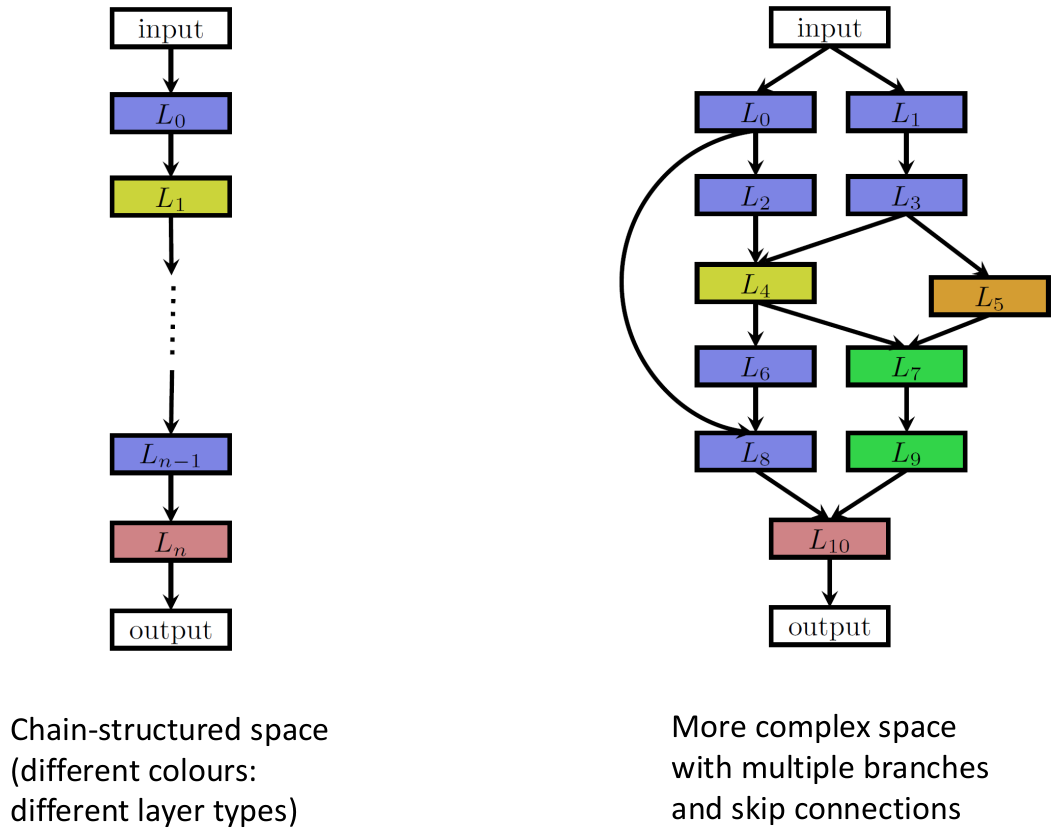
\includegraphics[height=\textheight]{images/lecture_frank/s25}
}
\end{frame}
%----------------------------------------------------------------------
%----------------------------------------------------------------------
\begin{frame}[c]{Cell Search Spaces}

{
	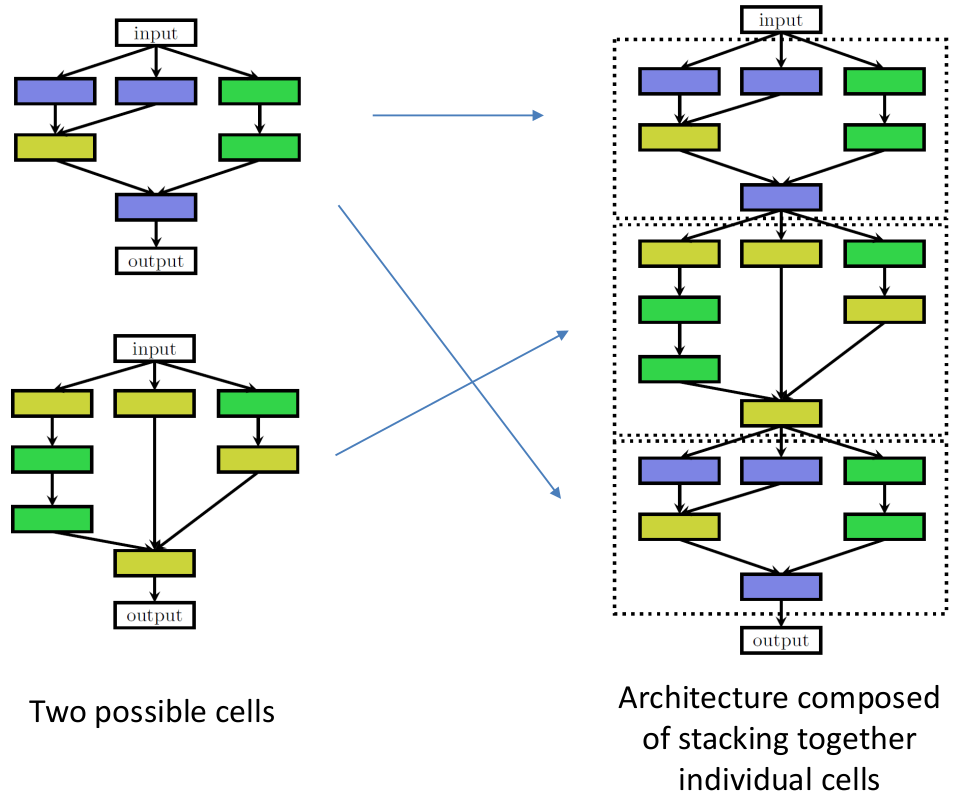
\includegraphics[height=.9\textheight]{images/lecture_frank/s26}
}
\end{frame}
%----------------------------------------------------------------------
%----------------------------------------------------------------------
\begin{frame}[c]{NAS as Hyperparameter Optimization}
\begin{itemize}
	\item Chain-structured space:
	\begin{itemize}
		\item Hyperparameters of layer $k$ conditional on depth $\geq k$
	\end{itemize}
	\item Cell search space
	\begin{itemize}
		\item Fixed (or maximum) number of nodes per cell (e.g., 5)
		\item For each: categorical choice between various operations, e.g.,
		between \{conv3x3, conv5x5, max pool, separable conv3x3, ...\}
	\end{itemize}
\end{itemize}
\end{frame}
%----------------------------------------------------------------------
%----------------------------------------------------------------------
\begin{frame}[c]{Outline}
\begin{itemize}
	\item Modern Hyperparameter Optimization
	\begin{itemize}
		\item AutoML as Hyperparameter Optimization
		\item Blackbox optimization
		\item AutoML Systems based on BlackBox Optimization
		\item Beyond Blackbox Optimization 
	\end{itemize}
	\item Neural Architecture Search
	\begin{itemize}
		\item Brief History
		\item Search Space Design
		\item[$\to$] Blackbox Optimization
		\item Beyond Blackbox Optimization
	\end{itemize}
\end{itemize}
\end{frame}
%----------------------------------------------------------------------
%----------------------------------------------------------------------
\begin{frame}[c]{Early Works on Neural Architecture Search}
\begin{itemize}
	\item Neuroevolution (already since the 1990s)
	\begin{itemize}
		\item Some authors used evolutionary algorithms for the
		architecture, optimizing the weights with SGD
		\item Others optimized both architecture and weights with
		evolutionary methods
	\end{itemize}
	\item Bayesian optimization
	\begin{itemize}
		\item Bergstra et al, 2013: optimized 238 hyperparameters of a vision
		architecture with TPE
		\item Mendoza et al, 2016: joint optimization of architecture and
		hyperparameters in Auto-Net, first Auto-DL system to win a
		competition dataset against human experts
	\end{itemize}
\end{itemize}
\end{frame}
%----------------------------------------------------------------------
%----------------------------------------------------------------------
{\setbeamertemplate{logo}{}
\begin{frame}[c]{Reinforcement Learning}
\begin{itemize}
	\item Reinforcement Learning \lit{Zoph \& Le, ICLR 2016}
	\begin{itemize}
		\item State-of-the-art results for CIFAR-10, Penn Treebank
		architecture, optimizing the weights with SGD
		\item Large computational demands \alert{800 GPUs for 2 weeks, 12.800 architectures evaluated}
		\item Hyperparameter optimization only as postprocessing
	\end{itemize}
\end{itemize}

{\centering
	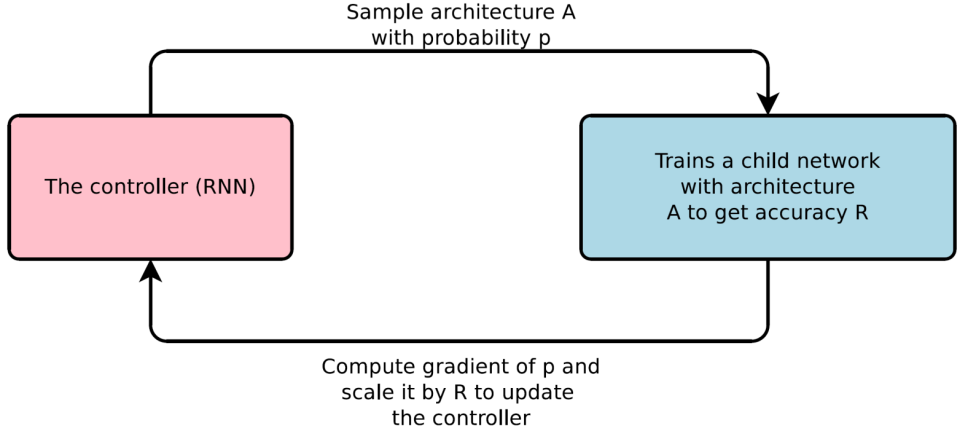
\includegraphics[width=\textwidth]{images/lecture_frank/s27}
}
\end{frame}
}
%----------------------------------------------------------------------
%----------------------------------------------------------------------
\begin{frame}[c]{Regularized / Aging Evolution}
\begin{itemize}
	\item Standard evolutionary algorithm \lit{Real et al, arXiv 2018}
	\begin{itemize}
		\item Oldest solutions are dropped from the population
		\begin{itemize}
			\item Even if they are the best performing ones
		\end{itemize}
		\item Very competitive results
	\end{itemize}
\end{itemize}

{\centering \hspace*{2.5cm}
	\includegraphics[width=.6\textwidth]{images/lecture_frank/s28}
}
\end{frame}
%----------------------------------------------------------------------
%----------------------------------------------------------------------
\begin{frame}[c]{Outline}
\begin{itemize}
	\item Modern Hyperparameter Optimization
	\begin{itemize}
		\item AutoML as Hyperparameter Optimization
		\item Blackbox optimization
		\item AutoML Systems based on BlackBox Optimization
		\item Beyond Blackbox Optimization 
	\end{itemize}
	\item Neural Architecture Search
	\begin{itemize}
		\item Brief History
		\item Search Space Design
		\item Blackbox Optimization
		\item[$\to$] Beyond Blackbox Optimization
	\end{itemize}
\end{itemize}
\end{frame}
%----------------------------------------------------------------------
%----------------------------------------------------------------------
\begin{frame}[c]{Main approaches for making NAS efficient}
\begin{itemize}
	\item Network morphisms \lit{Chen et al, ’16; Cai et al, ’17 \& ‘18;
		Elsken et al, ’17 \& 18}
	\item Weight sharing \lit{Pham et al,’18; Bender et al, ’18; Liu et al, ‘18}
	\item Multi-fidelity optimization \lit{Klein et al, ‘16; Li et al, ‘18;
		Falkner et al, ‘18}
	\item Meta-learning \lit{so far unexplored}
\end{itemize}
\end{frame}
%----------------------------------------------------------------------
%----------------------------------------------------------------------
\begin{frame}[c]{Network morphisms}
\begin{itemize}
	\item Network morphisms \lit{Chen et al, 2015; Wei et al, 2016; Cai et al, 2017}
	\begin{itemize}
		\item Change the network structure,
		but not the modelled function
		\item I.e., for every input the network yields the same output as
		before applying the network morphism
		\item Allow efficient moves in architecture space
	\end{itemize}
\end{itemize}
\end{frame}
%----------------------------------------------------------------------
%----------------------------------------------------------------------
\begin{frame}[c]{Fast Architecture Search via Network Morphisms}

{\centering
	\includegraphics[width=\textwidth]{images/lecture_frank/nash}
	Result: enables \alert{architecture search in 12 hours on 1 GPU}
}
\end{frame}
%----------------------------------------------------------------------
%----------------------------------------------------------------------
\begin{frame}[c]{Efficient Multi-objective Architecture Search}
\lit{Elsken, Metzen \& Hutter, arXiv 2018}
\begin{itemize}
	\item To trade off network size vs. error,
	maintain a \alert{Pareto front} of the \alert{2 objectives}
\end{itemize}
{\centering
\includegraphics[width=\textwidth]{images/lecture_frank/s29}
}
\begin{itemize}
\item Evolve a population of Pareto-optimal architectures over time
\item \alert{LEMONADE}: Lamarckian Evolution for Multi-Objective Neural Architecture Design
\begin{itemize}
	\item Weight inheritance through approximate morphisms
	\item Still cheap: 1 week on 8 GPUs
\end{itemize}
\end{itemize}
\end{frame}
%----------------------------------------------------------------------
%----------------------------------------------------------------------
\begin{frame}[c]{Evolution of population of architectures}

{\centering \hspace*{1.25cm}
	\includegraphics[width=.8\textwidth]{images/lecture_frank/pnash}
}
\end{frame}
%----------------------------------------------------------------------
%----------------------------------------------------------------------
{\setbeamertemplate{logo}{}
\begin{frame}[c]{LEMONADE: generation of children}

{\centering \hspace*{1.25cm}
	\includegraphics[height=.9\textheight]{images/lecture_frank/moas-1}
}
\end{frame}
}
%----------------------------------------------------------------------
%----------------------------------------------------------------------
\begin{frame}[c]{LEMONADE: train. and eval. of architectures}

{\centering \hspace*{1.25cm}
	\includegraphics[height=.9\textheight]{images/lecture_frank/moas-2}
}
\end{frame}
%----------------------------------------------------------------------
%----------------------------------------------------------------------
{\setbeamertemplate{logo}{}
\begin{frame}[c]{Efficient Multi-objective Architecture Search}
\lit{Elsken, Metzen \& Hutter, arXiv 2018}
\begin{itemize}
	\item \alert{Comparison to existing mobile-sized networks}
	\begin{itemize}
		\item Using the same training pipeline
		\item Better than manually-constructed mobile architectures
		\item Better results than NASNet and 35x faster search (56 vs. 2000 GPU days)
	\end{itemize}
\end{itemize}
{\centering
\includegraphics[width=\textwidth]{images/lecture_frank/s30}
}
\end{frame}
}
%----------------------------------------------------------------------
%----------------------------------------------------------------------
{\setbeamertemplate{logo}{}
\begin{frame}[c]{Efficient Multi-objective Architecture Search}
\lit{Elsken, Metzen \& Hutter, arXiv 2018}
\begin{itemize}
	\item \alert{Comparison to existing mobile-sized networks}
	\begin{itemize}
		\item Using the same training pipeline
		\item Better than manually-constructed mobile architectures
		\item Better results than NASNet and 35x faster search (56 vs. 2000 GPU days)
	\end{itemize}
\end{itemize}
{\centering
	\includegraphics[width=\textwidth]{images/lecture_frank/s31}
}
\end{frame}
}
%----------------------------------------------------------------------
%----------------------------------------------------------------------
{\setbeamertemplate{logo}{}
\begin{frame}[c]{Weight Sharing}
\begin{itemize}
	\item Convolutional Neural Fabrics \lit{Saxena \& Verbeek, NIPS 2016}
\end{itemize}
{\centering
	\includegraphics[width=\textwidth]{images/lecture_frank/s32}
}
\end{frame}
}
%----------------------------------------------------------------------
%----------------------------------------------------------------------
{\setbeamertemplate{logo}{}
\begin{frame}[c]{DARTS: Differentiable Neural Architecture Search}
\begin{itemize}
	\item Instead of making discrete choices between operators:
	\begin{itemize}
		\item Use all the choices, with a continuous weight each
		\item This allows for computing gradients w.r.t. the weight
	\end{itemize}
\end{itemize}
{\centering
	\includegraphics[width=.95\textwidth]{images/lecture_frank/s33}
}
\end{frame}
}
%----------------------------------------------------------------------
%----------------------------------------------------------------------
\begin{frame}[c]{Summary by Learning Goals}
\begin{itemize}
	\item Having heard this lecture, you can ...
	\begin{itemize}
		\item Explain how AutoML can be formulated as a hyperparameter
		optimization problem
		\item List various contemporary HPO methods, along with advantages
		and disadvantages
		\item Describe how to use multi-fidelity methods to speed up HPO
		\item Describe different search spaces for neural architecture search
		\item Describe various blackbox optimization methods for NAS
		\item Explain various speedup techniques for NAS
	\end{itemize}
\end{itemize}
\end{frame}
%----------------------------------------------------------------------